\chapter{Theory and Methods of Plenoptic Imaging}
\markboth{\MakeUppercase{Theory and Methods of Plenoptic Imaging}}{}
\label{chap:chapter1}
\section{Introduction}
\label{sec:intro1}
A camera is a device that captures light in a scene \cite{zhou2011computational}. The main constituents of a conventional camera are the detector and lens. The rays of light passing through the aperture of the lens are recorded on the sensor as a two dimensional irradiance map of the scene imaged. Therefore a traditional camera performs a limited sampling of the complete set of rays and in general of the amount of information contained in the scene \cite{nayar2006computational}. Finding methods to quantify, extract and process the full set of information contained in the light field is a comnplex problem. The space is filled with a dense array of light with various intensities \cite{adelson1991plenoptic}. From each point of the object imaged a cone of rays departs and fills the whole space while propagating. If a traditional camera is placed at a certain position from the object it will sample only the rays passing through its aperture. The set of information contained in this cone of rays will then be recorded on a two dimensional plane. This process of recording light coming from a three dimensional scene on a two dimensional plane causes loss of information. Following Adelson and Bergen \cite{adelson1991plenoptic} all the information carried by the light propagating into space can be described by a function, called the plenoptic function. Different parametrizations of the plenoptic function are possible. One of these is a four dimensional function called Light Field that will be discussed in more detail in the next sections. A new class of optical instruments, called computational cameras are also described; these are able to record and extract information from the light field. Computational cameras differ form a conventional camera in the way they sample the light coming from the object using a non conventional new optics that codifies the light that hits the detector. This coded information is then decoded by a computational stage, in order to extract an image \cite{nayar2006computational}. Schematics of the difference between a conventional and a computational camera can be found in figure \ref{fig:systems}
\begin{figure}[H]
	\centering
	\includegraphics[width=.7\textwidth]{systemsNew.eps}
	\caption{\label{fig:systems}Differences between a traditional camera and a computational camera \cite{nayar2006computational}.}
\end{figure}
\section{Plenoptic Function and the Light Field}
\label{sec:lightfield}
A grayscale photograph taken by a conventional camera represents the intensity of light seen by a single viewpoint, at a single time, averaged and weighted over the wavelengths of the visible spectrum \cite{adelson1991plenoptic}. The term viewpoint is used to identify a direction of view of the scene. For each point of the sensor, the intensity can be represented as function of the position $P(x,y)$. A colour photograph adds information about the wavelength $\lambda$\nomenclature{$\lambda$}{Wavelength of the light} of the light adding a third variable, $P(x,y,\lambda)$. If several photos are taken in succession forming a movie the time dependence is added, $P(x,y,\lambda,t)$ and if the movie is captured using holographic techniques, i.e. saving phase and amplitude of the optical field, all the information regarding the light intensity observable form any viewpoint $\overrightarrow{V} = (V_x, V_y, V_z)$ is recorded. Therefore to describe all the information that is potentially available from the light coming from the object a seven dimensional function is needed. It takes the name of plenoptic function and its name comes from Latin \textit{plenum} that means full \cite{adelson1992single, adelson1991plenoptic,wetzstein2011computational}. The plenoptic function implicitly contains a description of every possible photograph that can be taken of a particular scene from any possible point of view. To record the plenoptic function, one should move the camera along all the possible positions $\overrightarrow{X}=(x, y, z)$ around the object and take a snapshot or have an array of cameras surrounding the object taking snapshots simultaneously. The plenoptic function is an idealized concept and it is impossible to record it completely. However it is possible to acquire samples of it or projections along one or more dimensions. For example a conventional grayscale picture is a two dimensional slice along the coordinates x and y of the seven dimensional plenoptic function taken from a single point of view, averaging the wavelength and integrating over the exposure time. A plenoptic camera is able to record a section of the plenoptic function \cite{adelson1991plenoptic}. In particular, it records the part of the plenoptic function whose rays pass through the aperture of the camera, hence all the possible viewpoints contained in the lens aperture. Final images are constructed by sectioning the plenoptic function along certain coordinates. The process of extracting information from the plenoptic function is called rendering \cite{levoy1996light,georgiev2010focused} and it is where the computational stage operates. 
Before proceeding in describing a plenoptic camera in detail it is useful to define another parametrization of the plenoptic function derived by Levoy and Hanrahan \cite{levoy1996light} that is more useful to implement the computational algorithms in the following sections. This parametrization is called light field and is the radiance as a function of position and direction \cite{levoy1996light}. It is described by a set of four coordinates, two spatial coordinates and two directional coordinates and for this reason is often referred to as the 4D Light Field. There are two possible representations of the light field: the two-point representation and the point-angle representation. With reference to figure \ref{fig:lightfield} in the two point parametrization a ray of light is propagating in the free space from the point \textit{(x,y)} to the point\textit{ (u,v)}. Its direction of propagation in the three dimensional space is defined by the two points where it crosses two parallel planes. Therefore the set of coordinates \textit{(x,y)} and \textit{(u,v)} defines only one ray of light \cite{levoy1996light}. The point angle parametrization instead uses the coordinates of the point where the ray intercepts a plane perpendicular to the optical axis, and the angles that it forms with the optical axis along the directions x and y, namely $\theta_x$ \nomenclature{$\theta$}{Angular coordinate} and $\theta_y$, as shown in figure \ref{fig:lightfield2} \cite{georgiev2006light}. In both cases the intensity is a function of four coordinates. \\ The 4D light field is therefore:
\begin{equation}
\label{eq:lightfield}
L(x,y,u,v) = L(x,y,\theta_x,\theta_y)
\end{equation}
\begin{figure}[H]
	\centering
	\includegraphics[width=.3\textwidth]{C:/Users/Massimo/Documents/Thesis/Thesis_PhD/lightfield.eps}
	\caption{\label{fig:lightfield}Two point representation of the light field. Each ray of light is uniquely defined by the coordinates of two points of interception.}
\end{figure}
\begin{figure}[H]
	\centering
	\includegraphics[width=.6\textwidth]{C:/Users/Massimo/Documents/Thesis/Thesis_PhD/lightfield2.eps}
	\caption{\label{fig:lightfield2}Point angle representation of the light field. A ray of light is uniquely defined by the coordinates of a point that belongs to a plane perpendicular at the optical axis z and by the angles $\theta_x$ and $\theta_y$ that it forms with the optical axis along the directions x and y.}
\end{figure}
For each pixel of the sensor of a plenoptic camera it is possible to determine these four coordinates. The information provided by the two extra directional coordinates enables a set of computational features such as 3D reconstruction, synthetic refocus, full depth of field and aberration correction \cite{ng2006digital}. Each of these features is possible after having decoded the light field with the computational stage as shown in figure \ref{fig:systems}.
\section{Plenoptic Camera}
\label{sec:plenoticcamera}
A plenoptic camera is a camera that records the 4D light field as described in equation \ref{eq:lightfield}. The version proposed and built by Adelson and Wang in 1992 \cite{adelson1992single} is composed of a main lens, a sensor and a micro lens array placed in front of the sensor \cite{adelson1992single}. The presence of the micro array enables the codification of the directional information on the sensor, as will be discussed in the next sections. This coded image represents the raw data of the plenoptic camera and it can be seen in figure \ref{fig:plenoptic1}: 
\begin{figure}[H]
	\centering
	\includegraphics[width=.6\textwidth]{C:/Users/Massimo/Documents/Thesis/Thesis_PhD/plenopticamera.eps}
	\caption{\label{fig:plenoptic1} Plenoptic camera and its fundamental components. The presence of the micro array allows to record the light field .}
\end{figure}
The optical performance of the camera depends on the array's design characteristic. The main issue with the micro lens array is its position with respect to the main lens and the sensor. Depending on where it is placed two types of cameras are possible:
\begin{itemize}
	\item if the main lens forms its image on the micro array and the sensor plane is conjugated with the main lens it is the first generation plenoptic camera, or plenoptic 1.0 \cite{ng2005light} as seen in figure \ref{fig:plenoptic2} top.
	\item if the main lens forms its image on a plane that is different from the micro array plane and the micro lenses image the main lens image plane on the sensor it is the focused plenoptic camera, or plenoptic 2.0 \cite{georgiev2010focused} as seen in figure \ref{fig:plenoptic2} bottom.
\end{itemize}
 In the next sections both configurations will be extensively analysed and the way in which they capture the light field will be explained with particular attention to the differences in the raw data they produce. Their performances in term of lateral and directional (or angular) resolution will be detailed. The computational algorithms to render images from the raw data will also be extensively explained.
\begin{figure}[H]
	\centering
	\includegraphics[width=.4\textwidth]{C:/Users/Massimo/Documents/Thesis/Thesis_PhD/plenoptic10.eps}
	\caption{\label{fig:plenoptic2}Top: Plenoptic camera 1.0. The main lens is focused on the object and forms an image on the micro array. $f$ is the focal length of the main lens and $f_\mu$ the focal length of the micro lens array. Bottom: Plenoptic camera 2.0. The main lens is focused on an object and forms an image on the plane represented by the dashed line. The micro array acts as a relay between the main lens image and the sensor, satisfying the lens equation $1/a+1/b=1/f_\mu$.}
\end{figure}
\section{Plenoptic Camera 1.0}
\label{sec:camera10}
The first version of the plenoptic camera has been proposed and realised by Adelson and Wang in 1992 \cite{adelson1992single} and then improved by Ng $et al.$ \cite{ng2005light} and by Ng \cite{ng2006digital}in 2005-6.\\ The purpose of Ng was to design a camera that can use ray tracing techniques to compute synthetic photographs after the acquisition of the four dimensional light field. The main difference between Ng's camera and Adelson and Wang's camera is that the latter was a prototype that utilized a system of relay lenses from the main lens image plane and the micro lens array \cite{ng2005light} while in Ng's camera the array of micro lenses is placed directly in front of the sensor. Each micro lens forms an elemental sub image on the sensor and the directional information is contained inside the sub images. The main lens focuses the rays coming from one point on the object plane on a single point in the image plane. If an array of micro lenses is placed at this image plane all the rays will end up on a single micro lens. The micro lens will then split this bundle of rays on the sub image underneath it, separating the rays according to their direction. This is explained in figure \ref{fig:plenoptic3} where the plenoptic camera is modelled as a simple 2 f system. This behaviour can be achieved also using an array of pinholes instead as proposed originally by Yves. The problem using pinholes is that the amount of light reaching the sensor is considerably lower since a pinhole is restricting the energy output. Since the sensor plane is conjugate with the main lens under each micro lens there will be an image of the main lens aperture. For simplicity in figure \ref{fig:plenoptic3} the system is composed of only five micro lenses and each sub image is composed of only three pixels. The rays departing from a single point in the object plane shown in blue, red and green, are transferred by the main lens on a single micro lens. As an effect of the micro lens, each ray ends on a different pixel of the micro image.
\begin{figure}[H]
\centering
\includegraphics[width=.9\textwidth]{C:/Users/Massimo/Documents/Thesis/Thesis_PhD/raypleno10.eps}
\caption{\label{fig:plenoptic3}Ray diagram of a plenoptic 1.0 system. The main lens is in a 2f configuration and the sensor plane is conjugated with the main lens plane. The micro lens position maps the position (x,y) of the point P, while the sub image maps the directions of the rays coming from that point. The ray with direction $\theta_1$ falls on the pixel 1 (blue), the ray with direction $\theta_2$ falls on the pixel 2 (green) and the ray with direction $\theta_3$ falls on the pixel 3 (red). The sub image $d$ maps the direction of the rays.  }
\end{figure}
Since in the simplified case of figure \ref{fig:plenoptic3} there are only three pixels per micro lens, the maximum number of directions that can be sampled is three. A plenoptic camera samples as many directions as the number of pixels under each lenslet, therefore the directional resolution is given by the sub image resolution. Figure \ref{fig:plenoptic3} also shows that the spatial position of the point P is recorded at the micro array plane and the sampling of the position is linked to the number of lenses in the micro array. This leads to a trade-off between directional and spatial resolution since due to the finite dimension of the sensor, when more pixels are used to record the direction the same amount of pixels are lost to record the position. \\
With reference to figure \ref{fig:plenoptic4} two points are shown at two different positions on the same focal plane. The task now is to find a link between Levoy's and Hanrahan's two point representation of Light Field \cite{levoy1996light,levoy2006microscope} and the output data of the plenoptic 1.0 camera. Each sub image under each lenslet is an image of the main lens aperture, while the main lens image is formed on the micro array plane. To define the direction of a ray two points are needed. One point is its origin, the second is where it crosses the main lens. These two points are sampled by the lenslet array and by the sub images on the sensor, as shown in figure \ref{fig:plenoptic4}. Therefore it is possible to refer to the micro lens position on the array with spatial coordinates (x,y), and to the pixels of the sub images as the directional coordinates (u,v). With an array of 5 $\times$ 5 micro lenses and a sensor of 15 $\times$ 15 pixel, the 4D light field recorded will be a 5 $\times$ 5 $\times$ 3 $\times$ 3 function. Each point of this function is an intensity value identified by four coordinates, 2 spatial and 2 directional. the sampling of the spatial coordinates is 5 $\times$ 5, the sampling of the directional coordinates is 3 $\times$ 3. 
\begin{figure}[H]
	\centering
	\includegraphics[width=.7\textwidth]{C:/Users/Massimo/Documents/Thesis/Thesis_PhD/plenoray2.eps}
	\caption{\label{fig:plenoptic4} Sampling of Light Field. Each ray is described by a set of four coordinates, two spatial (x,y) and two directional (u,v). The spatial coordinates are sampled by the position of the lenslet in the micro array, the directional coordinates are sampled by the pixel under the lenslet.}
\end{figure}
This sampling used in the example above is of course very low. The amount of light captured by a lens is defined by its f-number that is the ratio between the focal length and the aperture diameter. The f-number is proportional to the number of rays with different directions that enter into the main lens aperture diameter. The relative f-number can also be defined as the ratio of the distance between the lens and its image and the aperture diameter. 
\begin{equation}
\label{eq:f_num}
f_{\#} = \dfrac{v}{d}
\end{equation} 
where $v$ is the distance from the main lens and the image plane and $d$ its aperture diameter. Another useful quantity to describe the amount of directions sampled by a lens is its numerical aperture, defined, referring to figure \ref{fig:plenoptic5} as:
\begin{equation}
\label{eq:NA}
NA=n sin(\theta)\simeq n \theta =\dfrac{2}{f_{\#}}
\end{equation}
Where $n$ is the index of refraction, and $\theta$ is half the total range of directions sampled by the lens. The assumption of dealing with small angles was made because the distance from $u$ between the main lens and the micro array is bigger than the diameter of the micro lens. In air, n=1, therefore the relation between the f-number and the range of directions is given by:
\begin{equation}
\label{eq:fnum1}
\Delta\theta= 2\theta=\dfrac{4}{f_{\#}}
\end{equation}
 To be sure that all the directions sampled by the main lens are mapped into the light field, the f-number of the lenslet should match the f-number of the main lens \cite{ng2005light} as shown in figure \ref{fig:plenoptic5}. This condition known as f-number matching is very important in plenoptic imaging. If the f-number of the lenslet is smaller than the one of the main lens then there is an under sampling of the rays intercepted by the main aperture, since some of the pixels remain dark. If the f-number of the lenslet is bigger there is cross-talk between the sub images. In both cases directional information is in part lost (figure \ref{fig:plenoptic7}) .
\begin{figure}[H]
	\centering
	\includegraphics[width=.7\textwidth]{C:/Users/Massimo/Documents/Thesis/Thesis_PhD/fnumbermatching.eps}
	\caption{\label{fig:plenoptic5}F-number matching between the main lens and the micro lens in the array.  }
\end{figure}
\begin{figure}[H]
	\centering
	\includegraphics[width=.7\textwidth]{C:/Users/Massimo/Documents/Thesis/Thesis_PhD/fnumber2.eps}
	\caption{\label{fig:plenoptic7}When the f-number is matched, all the rays captured by the main lens are mapped on the sub image (yellow). If the f-number of the lenslet is smaller (red), the sub image is smaller and there is an under sampling of the set of rays. If the f-number of the lenslet is bigger (green), the sub image is larger and cross talk happens between neighbouring sub images .  }
\end{figure}
\newpage
\subsection{Phase Space in Plenoptic 1.0}
\label{sec:phase_space}
It is useful to analyse the sampling of the light field from a phase space point of view. In figure \ref{fig:plenoptic6} a point source is sampled by the lenslet array.\\
 The one dimensional case is considered here for simplicity. The single ray departing from the point P on the focal plane of the main lens is refracted by the optical system and is captured by a pixel on the sensor that belongs to the sub image of a lenslet. The sub image position on the array gives the coordinate x. The pixel of the sub image gives the direction $\theta_x$. Therefore in the phase space a single ray is represented by a point with coordinates (x, $\theta_x$).
Considering all the rays departing from the point \textit{P(x)} captured by the main lens, they will all be focused on a single lenslet and then split on the sub image. Each pixel of the sub image corresponds to a different direction (ray). In the phase space this is equivalent to a vertical line. The physical meaning is that for a single spatial position \textit{x} corresponds a range of $\Delta \theta_x$ possible different directions, defined by the numerical aperture of the main lens matched with the one of the lenslet.\\
\newpage
\begin{figure}[H]
	\centering
	\includegraphics[width=.9\textwidth]{C:/Users/Massimo/Documents/Thesis/Thesis_PhD/phasespace10.eps}
	\caption{\label{fig:plenoptic6}Sampling of the light field and phase space representations of the rays.  }
\end{figure}
\newpage
\subsection{Light Field Parameterization}
\label{sec:LFparam}
Before discussing the rendering procedures for plenoptic 1.0 light field data, the three different parametrizations of the light field from the raw image will be described. A plenoptic 1.0 raw image looks like an array of sub images, each sub image contains samples of direction. An example of a plenoptic raw image can be seen in figure \ref{fig:rawlena10}. The raw image has been generated by simulating light propagating into a plenoptic camera, using a Matlab toolbox developed as part of this work which is described in detail in chapter \ref{chap:fresnel}. The simulated camera is composed of a 60 mm focal length lens, with an aperture of 7 mm, and a sensor with a resolution of 1500 $\times$ 1500 pixels. The micro array is composed of 75 $\times$ 75 lenslet with a focal length of 5 mm. The object imaged is a flat two dimensional image, therefore no depth information is stored. The reason for using flat objects to test a plenoptic imaging system is due to the fact that at this point of the work the interest is focussed on  understanding how the directions of the ray of light are recorded on the sensor, therefore reducing the degree of freedom of the problem to a flat isotropic isotropically emitting object simplifies the understanding of the problem. In the next chapters more accurate simulations will be presented taking into account the depth.
\begin{figure}[H]
	\centering
	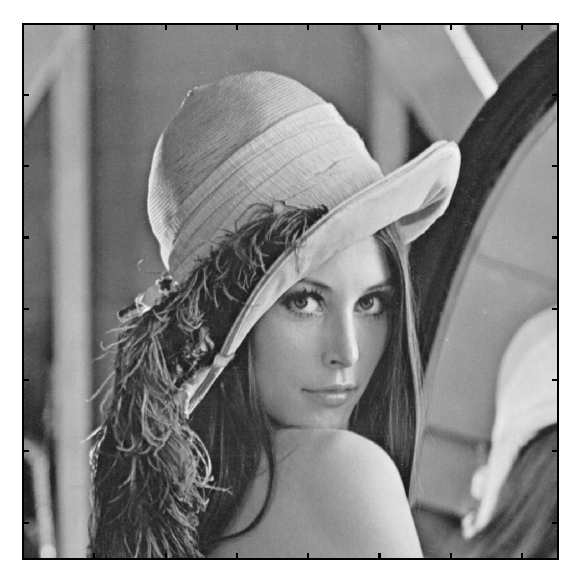
\includegraphics[width=.5\textwidth]{C:/Users/Massimo/Documents/Thesis/Thesis_PhD/lena_full.eps}
	\caption{\label{fig:lenafull} Image used as an object in the simulations.}
\end{figure}
\begin{figure}[H]
	\centering
	\includegraphics[width=.9\textwidth]{C:/Users/Massimo/Documents/Thesis/Thesis_PhD/rawlena.eps}
	\caption{\label{fig:rawlena10}Left: Example of a raw plenoptic 1.0 image. Right: Zoom on the raw image of the region indicated with the red square. Each lenslet is formed by 20 $\times$ 20 pixels. Each pixel represents a direction of the rays hitting the lenslet that produced the sub image.  }
\end{figure}
This raw image is the first parameterization of the light field and it is called the camera view. Pixels are arranged according to the positional coordinates, and each sub image contains the directional coordinates as shown in figures \ref{fig:rawlena10} and \ref{fig:arrayview}. \\
A second parameterization, known as the array view, is obtained by rearranging the pixels according to the directional coordinates \cite{ng2006digital}. The result is an array of N $\times$ N sub images, where N is the number of samples of the directional coordinates. Each sub image represents the point of view linked with a direction $(\theta_x, \theta_y)$. The array view can be seen in figure \ref{fig:arrayview1} and \ref{fig:arrayview1z} while the method to pass from the camera view to the array view is illustrated in figure \ref{fig:arrayview}. \\
\begin{figure}[H]
	\centering
	\includegraphics[width=.9\textwidth]{C:/Users/Massimo/Documents/Thesis/Thesis_PhD/imgformation.eps}
	\caption{\label{fig:arrayview}The array view is an array of the different point of view obtained rearranging the pixels according to the directional coordinates.  }
\end{figure}
An example of the array view parametrization of the raw image in figure \ref{fig:rawlena10} is shown in figure \ref{fig:arrayview1}.\\
The third and last parametrization of the light field is the 4-D radiance, a four dimensional function that represents radiance as a function of position and direction. \cite{levoy1996light}. This third parametrization is less intuitive but is very useful from a computational point of view since it is a four dimensional array, and every ray can be addressed by a set of four coordinates, or indices, as will be explained in detail in chapter \ref{chap:chapter4}.
\newpage
\begin{figure}[H]
	\centering
	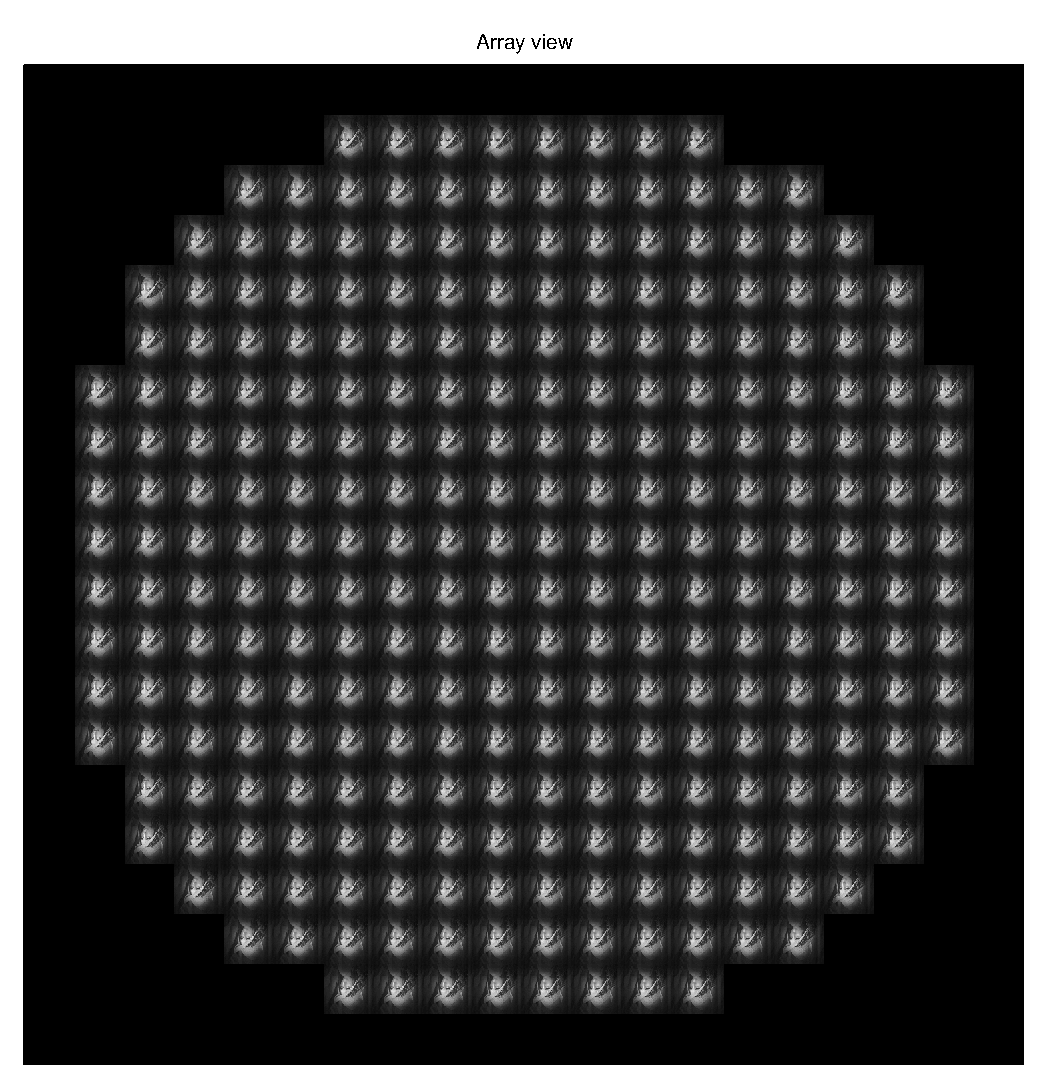
\includegraphics[width=.6\textwidth]{C:/Users/Massimo/Documents/Thesis/Thesis_PhD/arrayview.eps}
	\caption{\label{fig:arrayview1}Array view of the raw data shown in figure \ref{fig:rawlena10}.  }
\end{figure}
\begin{figure}[H]
	\centering
	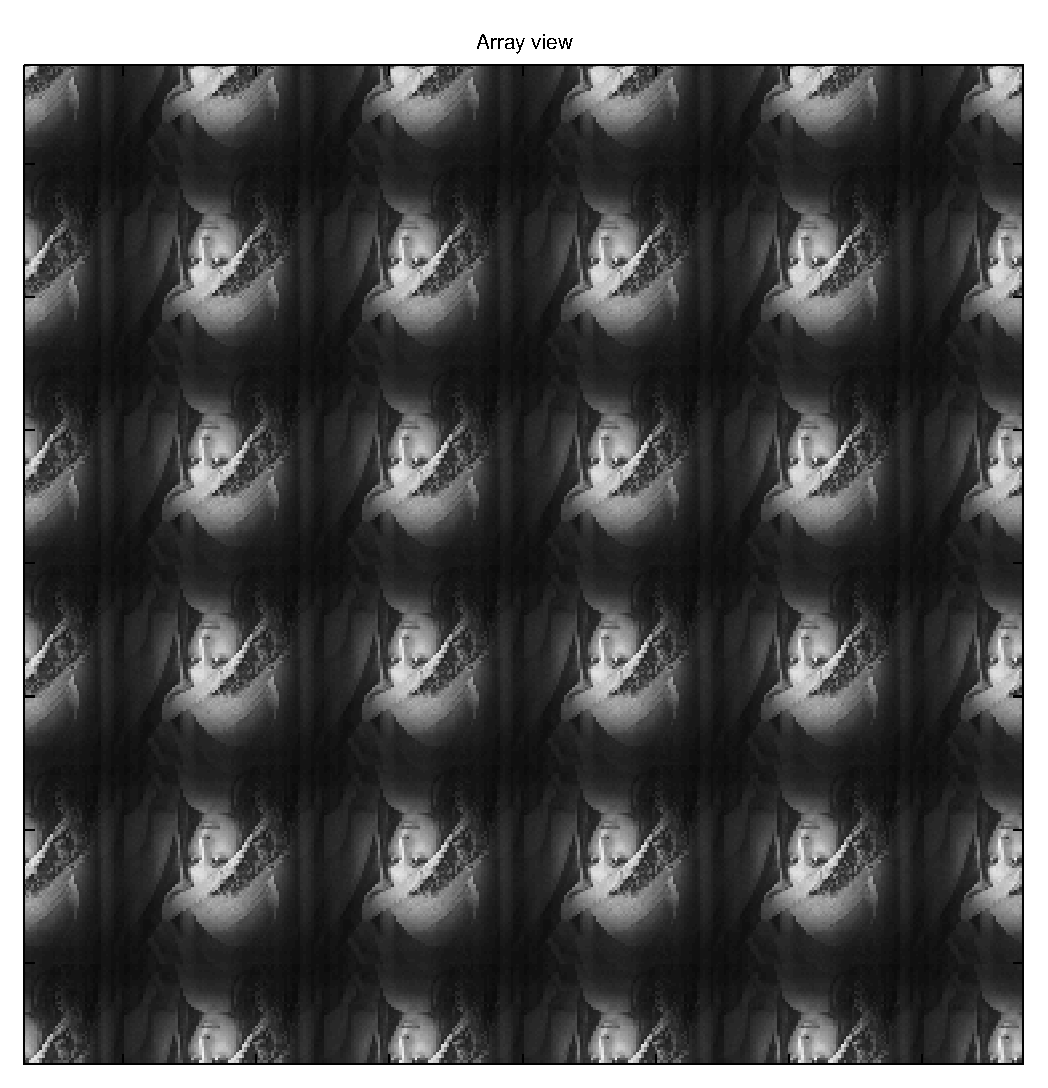
\includegraphics[width=.6\textwidth]{C:/Users/Massimo/Documents/Thesis/Thesis_PhD/arrayviewz.eps}
	\caption{\label{fig:arrayview1z}Zoom of the central part of the array view showing in detail the different points of views.  }
\end{figure}
\newpage
\section{Plenoptic 1.0 Rendering}
\label{sec:rendering1}
The act of de-codifying the information present on the sensor of the plenoptic camera in order to get an image is called rendering. 
In a conventional 2D image the intensity of each single pixel, corresponding to a position, is obtained by summing the contributions of all the rays of light converging to that point of the sensor \cite{georgiev2010focused} as shown in figure \ref{fig:render1}. This is equivalent to integrating over all possible directions for each position. 
\begin{figure}[H]
	\centering
	\includegraphics[width=.5\textwidth]{C:/Users/Massimo/Documents/Thesis/Thesis_PhD/rendering1.eps}
	\caption{\label{fig:render1} The intensity of a single pixel is obtained summing all the rays of light coming from all the possible directions.\cite{ng2006digital} }
\end{figure}
The same is valid for a computational image, where the integrations are made in post processing from the raw plenoptic data captured.
 If $L(x,y,u,v)$ is the sampled 4D light field, the radiance $E(x,y)$ on a pixel \textit{(x,y)} of the final rendered image will be given by integrating all the rays coming from all the sampled directions \textit{(u,v)} for any fixed point\textit{ (x,y)}. Following the work of Ng \cite{ng2006digital}:
\begin{equation}
\label{eq:rendering1}
I(x,y)=\dfrac{1}{z^2}\iint L(x,y,u,v)\mathscr{A}(u,v)cos^4\theta dudv
\end{equation} 
Where $z$ is the distance between the main lens and the sensor, $\theta$ is the angle formed by the rays and the sensor normal to the sensor surface and $\cos^4\theta$ is the vignetting factor. It takes into account the fact that the total light illuminating the sensor  declines moving outward  from  the  centre  of  the  image. The result is a relative darkening of the image toward 
its borders. This phenomenon can be well described by the so called "cosine fourth" law \cite{kerr2007derivation}. $\mathscr{A}(u,v)$ is an aperture function that limits the directions upon which integration takes place to the ones included in the aperture of the main lens. In the paraxial approximation, the $cos^4\theta$ term can be dropped as well as the $1/z^2$ term and equation \ref{eq:rendering1} becomes:
\begin{equation}
\label{eq:rendering2}
I(x,y)=\iint L(x,y,u,v)\mathscr{A}(u,v) dudv
\end{equation}
From a computational point of view, since the samples are discrete, the double integral becomes as a sum along the directional coordinates u and v. The total intensity of each pixel of the rendered image is then the sum of the intensities of the pixels that form the corresponding sub image divided by the number of pixels in the sub image. For a light field with N $\times$ N directional samples, the intensity $I(x,y)$ is given by:
\begin{equation}
\label{eq:rendering3}
I(x,y) = \dfrac{1}{N^2}\sum_{i=0}^N\sum_{j=0}^N L(x,y,i,j)
\end{equation}
This can be seen in the phase space where each pixel of the final image is made by the mean of all N directional samples \cite{georgiev2010focused}, as shown in figure \ref{fig:rendering2}.
 \begin{figure}[H]
 	\centering
 	\includegraphics[width=.5\textwidth]{C:/Users/Massimo/Documents/Thesis/Thesis_PhD/renderingphase.eps}
 	\caption{\label{fig:rendering2} Rendering an image from plenoptic 1.0 raw data is equal to summing all the directional samples for each position. This process is shown for the $(x,\theta_x)$ slice of the phase space. \cite{georgiev2010focused} }
 \end{figure}
 From figure \ref{fig:rendering2} it can be noted that rendering an image from a light field captured by a plenoptic 1.0 camera causes a loss of resolution compared with the image collected by a conventional camera using the full sensor. Each pixel of the final image corresponds to one lenslet. Considering a plenoptic camera composed of a sensor with a resolution of 1000 $\times$ 1000 pixels and a micro lens array of 100 $\times$ 100 lenslets, each sub image will contain 10 $\times$ 10 directional samples. All these samples will contribute in computing the intensity of a single pixel, therefore there will be only one pixel per lenslet in the final image whose resolution is 100 $\times$ 100 pixels. This is the main limitation to plenoptic 1.0 cameras: the better the directional information is sampled, the more spatial resolution is lost \cite{georgiev2010focused, ng2006digital}. An example of a rendered image from a computer generated light field is shown in figure \ref{fig:renderlena}
 \begin{figure}[H]
 	\centering
 	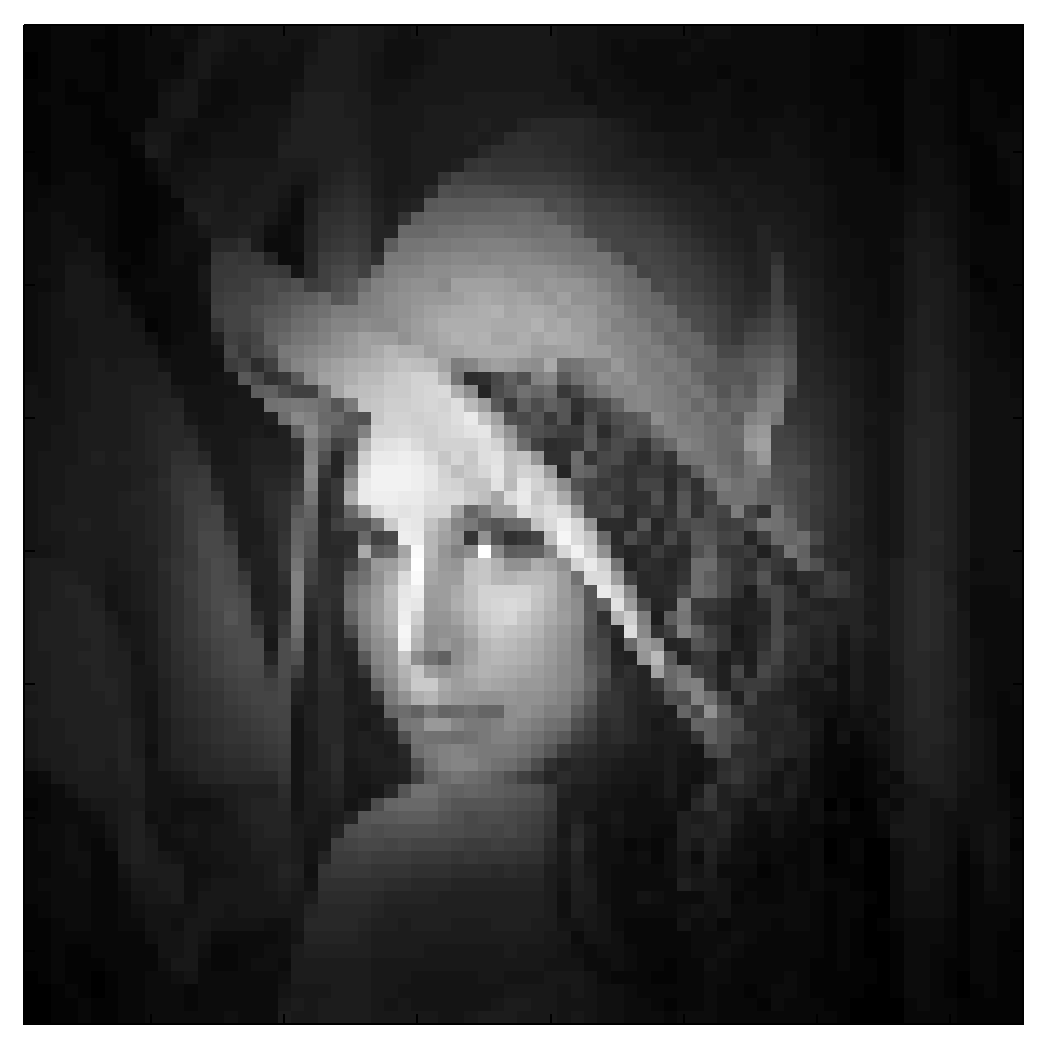
\includegraphics[width=.7\textwidth]{C:/Users/Massimo/Documents/Thesis/Thesis_PhD/renderlena.eps}
 	\caption{\label{fig:renderlena} rendered image from the raw data in figure \ref{fig:rawlena10}. Resolution is only 75 $\times$ 75 pixels.  }
 \end{figure}
 This loss of resolution arises from the fact that the lenslet array is not focused on the sensor and it produces on the sensor a blurred image \cite{georgiev2010focused}.
 \section{Plenoptic Camera 2.0}
 \label{sec:pleno20}
 A new kind of plenoptic camera, named focused plenoptic camera or plenoptic camera 2.0, has been proposed by Lumsdaine and Georgiev \textit{et al}. \cite{lumsdaine2008full,lumsdaine2009focused}. As shown in figure \ref{fig:plenoptic2} the plenoptic camera 2.0 is based on an array of micro lenses focused on the image plane of the main lens. In this configuration the sensor plane becomes conjugated with the main lens image plane. As will be discussed in the next sections, in a plenoptic 2.0 camera there is a flexible trade-off between angular and spatial resolution \cite{georgiev2010focused} leading to a full sensor resolution in the final image \cite{bishop2011full,georgiev2009resolution}. There are two possible configurations of the plenoptic 2.0 camera, as shown in figure \ref{fig:pleno201}. In both configurations each micro lens forms on the sensor a relay image of part of the main lens image. The position of the micro array is determined to satisfy the lens equation $1/a+1/b=1/f_{\mu}$, where $a$ is the distance from the main lens image plane to the micro array, $b$ is the distance from the micro array to the sensor plane and $f_{\mu}$ is the focal length of each micro lens. If $b$ is bigger than the focal length $f_{\mu}$ the camera is in a \textit{Copernican configuration} where the main lens image is a real image in front of the micro array, while if $b$ is smaller then $f_{\mu}$, the distance \textit{a} happens to be negative and the main lens image is formed behind the sensor plane. This is called \textit{Galilean configuration} and the micro array images a virtual main lens image (figure \ref{fig:pleno201}) \cite{georgiev2010focused}. 
 \begin{figure}[H]
 	\centering
 	\includegraphics[width=.7\textwidth]{C:/Users/Massimo/Documents/Thesis/Thesis_PhD/plenoptic201.eps}
 	\caption{\label{fig:pleno201} If the main lens image is formed in front of the micro array the configuration is called \textit{Copernican}, top, and the focal length of the micro array is smaller then the distance b. If the main lens image is formed behind the micro array the configuration is \textit{Galilean}, on the bottom, and the focal length of the micro array is bigger then the distance b. }
 \end{figure}
 For both configurations the magnification of the micro array stage is:
 \begin{equation}
 \label{eq:pleno20}
 m=\dfrac{b}{a}
 \end{equation}
 The ratio between the distances $a$ and $b$ plays a crucial role in sampling the light field in the plenoptic camera 2.0. Figure \ref{fig:rawpleno20} shows a raw plenoptic 2.0 image of a point source acquired through simulation (as discussed in chapter \ref{chap:fresnel}). The system is composed of a main lens with a focal length of 60 mm, in a 2f configuration and a micro array made of $150 \mu m$ diameter lenslets with focal length of 5.3 mm. The distances \textit{a} and \textit{b} are set in order to have a magnification \textit{m} of 0.3. In this configuration each point of the main lens image is sampled by three lenslets and each sub image corresponds to a point of view of the object. The number of points of view depends on the magnification of the micro array stage. Hence, in order to have more than one point of view recorded it is necessary that the magnification \textit{m} is less than one. Looking at figure \ref{fig:rawpleno20} the raw image is composed of a 3 $\times$ 3 matrix of sub images, three points of view in the x direction and three along the y direction. Figure \ref{fig:rawpleno203} shows central 5 $\times$ 5 sub images in the raw data. The central sub image records the direction corresponding to the central point of view, indicated in both figures with the number 2. The lenslets on the left and on the right of the central one record the directions corresponding to the point of views from the left, indicated with 1 in figure \ref{fig:rawpleno202}, and right, indicated with 3. The sub images 1 and 3 are shifted towards the outer edge of the sub image. This happens as an effect of the change in the point of view as well as because the sub images are flipped upside down as a consequence of the imaging law.
  \begin{figure}[H]
 	\centering
 	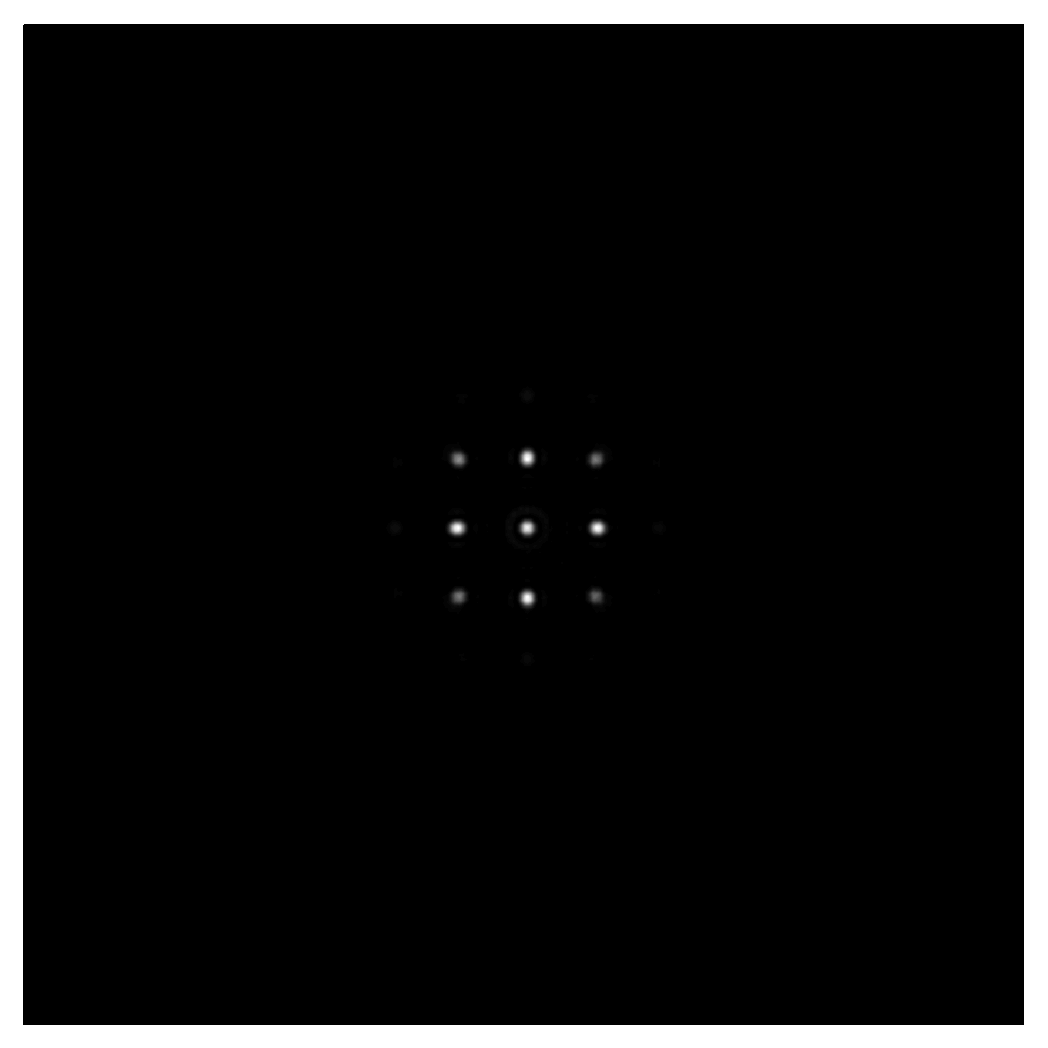
\includegraphics[width=.5\textwidth]{C:/Users/Massimo/Documents/Thesis/Thesis_PhD/rawimage.eps}
 	\caption{\label{fig:rawpleno20} Raw data of a point source sampled by a plenoptic 2.0 system with a magnification of the micro array stage equal to 0.3. Data acquired with numerical simulations. }
 \end{figure}
 \begin{figure}[H]
 	\centering
 	\includegraphics[width=.5\textwidth]{C:/Users/Massimo/Documents/Thesis/Thesis_PhD/rawzoom.eps}
 	\caption{\label{fig:rawpleno203} Zoomed raw data of a point source sampled by a plenoptic 2.0 system with a magnification of the micro array stage equal to 0.3. Data acquired with numerical simulations. The grid represent the boundaries of each sub image to show how the point of view of the point source changes across the lenslets. The sub images are shifted by a quantity proportional to the position of the lenslet in the array.  }
 \end{figure}
  \begin{figure}[H]
  	\centering
  	\includegraphics[width=1  	\textwidth]{C:/Users/Massimo/Documents/Thesis/Thesis_PhD/LFsampling.eps}
  	\caption{\label{fig:rawpleno202}Sampling of the light field by a plenoptic 2.0 system with a magnification of \textit{m=0.3}. For simplicity the one dimensional case is shown. Each micro lens has a diameter equal to d, a focal length $f_{\mu}$, and images the main lens image on the sensor according to the lens law $1/a+1/b=1/f_{\mu}$ The total range of directions that can be sampled is given by $d/b$. Each lenslet samples a sub set of directions equal to $d/a$ as a single direction. The range of directions shown in red are sampled by the central micro lens as a single point of view. The angular resolution is therefore \textit{d/a} and the total number of directional samples is \textit{a/b = 1/m}. In the specific case shown is 3. }
  \end{figure}
  As in the 1.0 case, the f-number of the micro lenses matches the f-number of the main lens.
 With reference to figure \ref{fig:rawpleno202} because of the f-number matching condition the total number of directions captured by the main lens is defined as $\Theta=D/z_2=d/b$ where D is the aperture of the main lens, $z_2$ the distance of the main lens image, d is the diameter of the lenslet and b is the distance between the lenslet and the sensor. The amount of directions captured by a single lenslet is equal to $p=d/a$. Hence the range sampled by the single lenslet with respect to the total range of directions in the light field is:
 \begin{equation}
 \label{eq:magnification}
 \dfrac{p}{\Theta}=\dfrac{d}{a}\dfrac{b}{d}=m
 \end{equation} 
 Hence:
  \begin{equation}
  \label{eq:magnification2}
  p=\dfrac{b}{a}\Theta=m\Theta
  \end{equation}
  Therefore the magnification of the lenslet array determines the angular resolution of the plenoptic 2.0 system. In the case illustrated in figures \ref{fig:rawpleno201} and \ref{fig:rawpleno202} for each position x on the main lens image plane, 3 directions are sampled. Since the main lens image is scaled by the lenslets by a factor of $m$, the resolution of the rendered image will be $b/a$ times the resolution of the full sensor. This fact implies that the spatio-angular trade off of the plenoptic 2.0 camera is not fixed by the number of micro lenses, but it is determined by the optical geometry of the micro lens stage, and is fully determined by the magnification $m=b/a$. The more samples of the directional coordinates, the less will be the spatial resolution of the rendered image. In section \ref{sec:phase2.0} a more rigorous proof of this will be given.
  Figure \ref{fig:rawpleno201} shows the effect of magnification on the raw image of a point source. If the magnification is 1, the main lens image is replicated on the sensor under only one lenslet. No further information is given by the micro array stage. The whole range of directions is sampled by a single lenslet and with only one point of view it is not possible to recover the directional information. In order to have more than one point of view, \textit{m} should be at least 0.5. In this case the point source is replicated under a total of four lenslets giving 2 $\times$ 2 points of view to render the image. If the magnification decreases further, the number of points of view increases. The directional information in plenoptic 2.0 is recorded not by a single lenslet like in the 1.0 case, but across many lenslets, since each point of the object plane is imaged by a number of lenslets proportional to the inverse of the magnification \ref{eq:pleno20}. Each lenslet samples a part of the directional coordinates contained into the solid angle \textit{d/a}. The more point of view that are present, the smaller will be the solid angle \textit{d/a}, and therefore, the better will be the angular resolution. \cite{lumsdaine2009focused}
   \begin{figure}[H]
  	\centering
  	\includegraphics[width=.8\textwidth]{C:/Users/Massimo/Documents/Thesis/Thesis_PhD/rawimages.eps}
  	\caption{\label{fig:rawpleno201}Raw images of a point source simulated with different magnifications. From top left to bottom right: \textit{m = 1, m = 0.5, m= 0.25, m = 0.1}. }
  \end{figure}
  \newpage
  \section{Plenoptic Camera 2.0: a Geometrical Optics Analysis}
  \label{sec:phase2.0}
  This section provides a mathematical proof of the concepts introduced in section \ref{sec:pleno20}. The mathematical model of Light Field sampling in plenoptic 2.0 has been developed by Lumsdaine and Georgiev \cite{lumsdaine2009focused,lumsdaine2008full}. The goal of this chapter is to express the intensity profile present on the sensor as a function of the light field at the focal plane of the main lens. The intensity on the sensor is given by integrating for each pixel along all the rays, or the directions, the radiance captured by the sensor in analogy with what was discussed in \ref{sec:rendering1}:
  \begin{equation}
 	\label{eq:phase201}
 	I(x,y)=\iint_{\theta_x, \theta_y}L(x,y,\theta_x,\theta_y) d\theta_xd\theta_y
  \end{equation} 
  For simplicity only one positional coordinate \textit{x} is considered, and its corresponding direction will be described by a new coordinate called \textit{momentum}, in analogy with Hamiltonian mechanics, defined as:
  \begin{equation}
	\label{eq:momentum2}
	p_x = n\theta_x
  \end{equation}
  where \textit{n} is the refractive index of the medium of propagation, assumed to be homogeneous. The reason of this change in coordinates is that using the momentum \textit{p} the transformations matrix of the optical elements are invertible and the calculations are simpler \cite{guillemin1990symplectic}. The one dimensional intensity profile is then equal to:
  \begin{equation}
  \label{eq:1Dintensity}
  I(x)=\int_{p_x}L(x,p_x) dp_x
  \end{equation} 
  In the phase space the rays composing the light field, will be represented by points with coordinates $(x,p_x)$. Given a ray $\overrightarrow{X_0}=(x,p_x)$, it is possible to define a ray transfer matrix \textit{A} describing the transformation the ray undergoes while propagating in an optical system as:
  \begin{equation}
  \label{eq:transmatrix1}
  \overrightarrow{X_1}=A\overrightarrow{X_0}
  \end{equation}
  Where $\overrightarrow{X_1}$ is a vector representing the ray after the transformation \textit{A}. The transformation matrix has the property of having its determinant equal to unity, \textit{det(A)=1}, and is invertible. It is therefore possible to express the ray $\overrightarrow{X_0}$ as a function of $\overrightarrow{X_1}$ as:
   \begin{equation}
   \label{eq:transmatrix2}
   \overrightarrow{X_0}=A^{-1}\overrightarrow{X_1}
   \end{equation}
   The same considerations can be made for the full set of rays composing the light field. In the assumption of zero loss during the propagation, the total light field \textit{L} is conserved, and $L(\overrightarrow{X_0})$ equals $L(\overrightarrow{X_1})$. Therefore:
   \begin{equation}
   \label{eq:transmatrix3}
   L_1(\overrightarrow{X_1})=L_0(\overrightarrow{X_0})
   \end{equation} 
   Because of equation \ref{eq:transmatrix1} the Light Field at the position $\overrightarrow{x_1}$ is :
   \begin{equation}
   \label{eq:transmatrix4}
   L_1(A\overrightarrow{X_0})=L_0(\overrightarrow{X_0})
   \end{equation}
   For the ray $\overrightarrow{X_1}=A\overrightarrow{X_0}$:
   \begin{equation}
   \label{eq:transmatrix8}
   L_1(\overrightarrow{X_1})=L_0(A^{-1}\overrightarrow{X_1})
   \end{equation}
   For the generic ray $\overrightarrow{X}$ the light field transformation formula becomes:
   \begin{equation}
   \label{eq:transmatrix5}
   L_1(\overrightarrow{X})=L_0(A^{-1}\overrightarrow{X})
   \end{equation}
   Equation \ref{eq:transmatrix5} shows the link between the light field at a plane, with the same light field after an arbitrary optical transformation.
     With reference to figure \ref{fig:basystem} a single lenslet of diameter \textit{d} is shown and the light field at the sensor plane $L_b(x,p_x)$ is expressed as a function of the coordinates of the light field at the main lens image plane $L_a(x,p_x)$. The link between the two light fields is given by equation \ref{eq:transmatrix5}. According to geometrical optics, and as is explained in Georgiev \textit{et al.}\cite{georgiev2011plenoptic}, the optical transfer matrix $A_{ab}$ from the main lens image plane and the sensor is the composition of two free space propagation matrices and a lens matrix.
      \begin{figure}[H]
      	\centering
      	\includegraphics[width=.7\textwidth]{C:/Users/Massimo/Documents/Thesis/Thesis_PhD/singlelens.eps}
      	\caption{\label{fig:basystem} System formed by a single lenslet. The rays at the main lens image plane are transformed into the rays at the sensor plane by the lenslet. The transformation can be described by a matrix \textit{A}. }
      \end{figure}
Therefore:
   \begin{equation}
   \label{eq:transmatrix6}
   A_{ab}=
   \begin{bmatrix}
   1 & b \\ \\
   0 & 1
   \end{bmatrix}
   \begin{bmatrix}
  1 & 0 \\ \\
  -\dfrac{1}{f_{\mu}} & 1
   \end{bmatrix}
   \begin{bmatrix}
   
   1 & a \\ \\
   0 & 1
   \end{bmatrix}
   =
   \begin{bmatrix}
   -\dfrac{b}{a} & 0\\\\
   -\dfrac{1}{f_{\mu}}&-\dfrac{a}{b}
     \end{bmatrix}
   \end{equation}
   Its inverse is:
   \begin{equation}
   \label{eq:transmatrix7}
   A_{ab}^{-1}=
   \begin{bmatrix}
   -\dfrac{a}{b} & 0\\\\
   \dfrac{1}{f_{\mu}}&-\dfrac{b}{a}
   \end{bmatrix}
   \end{equation}
     Applying the inverse $A^{-1}$ matrix to equation \ref{eq:transmatrix5} and substituting into the integral in equation \ref{eq:phase201}, the intensity on the sensor behind a single lenslet is: 
   \begin{equation}
   \label{eq:radiance}
   	I(x)=\int_{p_x}L_a(-\dfrac{a}{b}x,-\dfrac{b}{a}p_x -\dfrac{1}{f}x) dp_x
   \end{equation}
   From figure \ref{fig:basystem}, for a single spatial coordinate x on the main lens image plane the integration takes place on a range of directional coordinates $p_x$ equal to $d/b$ and the result is:
   \begin{equation}
   \label{eq:radiance2}
   I(x)=\dfrac{d}{b}L_a(-\dfrac{a}{b}x, -\dfrac{1}{b}x) 
   \end{equation}
   From equation \ref{eq:radiance2} the micro lens maps the spatial coordinates on the main lens image plane to the sensor with a scaling factor equal to the magnification $m=b/a$. Therefore the resolution of the sampled light field on the sensor is $b/a$ times the resolution of the sensor. The directional coordinates are mapped as $x/b$. If the lenslet diameter is $d$ then the maximum number of directional coordinates sampled by one lenslet is equal to the f-number of the lenslet $d/b$. Figure \ref{fig:basystem} shows how a single micro lens samples the radiance from a single point X on the main lens image plane. Each pixel of the micro lens image samples a single position X and a span of $d/a$ directional coordinates $p_x$. The same position X is sampled also by other micro-lenses as shown in figure \ref{fig:phaseba}, but since each micro lens only captures $d/a$ samples of the directional coordinates, each lenslet samples a different portion of the total span of directional coordinates contained in the light field.
   \begin{figure}[H]
   	\centering
   	\includegraphics[width=1\textwidth]{C:/Users/Massimo/Documents/Thesis/Thesis_PhD/smapling1.eps}
   	\caption{\label{fig:phaseba} Sampling of the light field by plenoptic 2.0 camera. For each of the two points represented, red and green, The total range of directional coordinates are sampled by three  different lenslets. For one position three directions are sampled, with a resolution of d/a. Therefore the directional sampling in plenoptic 2.0 is made across many lenslets. This can be seen in the phase space. Lenset B and C sample 2 directions indicated with the same number in the ray diagram and the phase space. Lens let A only samples one direction of the red point.   }
   \end{figure}
   \section{Plenoptic 2.0 Rendering}
   \label{sec:rendering201}
   The basic rendering in plenoptic 2.0 cameras is still made by integrating all directions associated to a single position, as shown \ref{eq:pleno20}. The difference with plenoptic 1.0 rendering is that this time the directional coordinates for a single position, $d/b$, are recorded across many lenslets, each sampling $d/a$ coordinates and as a consequence of that, the integration takes place across all of these micro lenses \cite{georgiev2006light}. The basic rendering process is shown in figure \ref{fig:render20}.
   \begin{figure}[H]
   	\centering
   	\includegraphics[width=.5\textwidth]{C:/Users/Massimo/Documents/Thesis/Thesis_PhD/rendering20b.eps}
   	\caption{\label{fig:render20} Image rendering with the focused plenoptic camera. One pixel of the rendered image is given by the integration on all the directions $d/b$ associated with a given position. The integration takes place across the lenslet and is represented by the vertical lines. Each lenslet is represented by the diagonal lines. }
   \end{figure}
   Rendering an image in plenoptic 2.0 is more complicated and less intuitive then the 1.0 case, therefore a more detailed analysis of plenoptic 2.0 rendering will be given in chapter \ref{chap:chapter5}.
   \section{Conclusions}
   In this chapter a general view of plenoptic imaging systems behaviour and characteristics was given. It is based on results already presented in the literature and it has the scope to put order in a new field where the literature is often fragmented and incomplete. It was introduced the concept of plenoptic function, as a function to describe the full set of information contained in the light. The concept light field was also presented as a four dimensional parametrization of the plenoptic function. Each ray of light is completely identified by a set of four coordinates, two spatial and two directional coordinates. This representation of the bundle of rays reaching the camera is very useful under a computational point of view since each ray of light can be represented as a point in the phase space. In the phase space an optical transformation is described by a optical transfer matrix with the property of having the determinant equal to one and to be invertible. In this way it is possible to give a mathematical description of the behaviour of the plenoptic camera and to put the basis for the ray tracing algorithms that will be presented in the following chapters.
   Two different types of plenoptic camera were described, the plenoptic 1.0 and 2.0. A detailed description of the how these two classes of devices record the light filed was given, pointing out the main differences in the performances of the two configurations.
   The main original contribution to the field given by this chapter is that for the first time a complete review of the characteristic of plenoptic camera 1.0 and 2.0 was given. This chapter represents a link between many pieces of work on plenoptic imaging and covers all the aspects of this new field providing a good overview of all the general aspects of plenoptic imaging.
   \nomenclature{$L$}{Light Field}
   \nomenclature{$x$}{Spatial coordinate}
   \nomenclature{$y$}{Spatial coordinate}
   \nomenclature{$z$}{Distance on the optical axis}
   \nomenclature{$v$}{Directional coordinate}
   \nomenclature{$u$}{Directional coordinate}
   \nomenclature{$a$}{Distance from the main lens image to the micro array}
   \nomenclature{$b$}{Distance from the micro array to the sensor}
   \nomenclature{$f$}{Focal length of the main lens}
   \nomenclature{$f_{\mu}$}{Focal length of the micro lens}
   \nomenclature{$d$}{Aperture diameter}
   \nomenclature{$\overrightarrow{X}$}{Vector representing the ray of light}
   \nomenclature{$A$}{Transformation matrix}
   \nomenclature{$A^{-1}$}{Transformation matrix}
   \nomenclature{$m$}{Magnification}
   \nomenclature{$D$}{Aperture diameter of the main lens}
   \nomenclature{$I$}{Intensity of the optical field}
   \nomenclature{$E$}{Radiance}